\documentclass[../BTOF_summary.tex]{subfiles}
 
\begin{document}

\section{The \btof\ Detector Hardware}

The \btofD\ consists of 16 elements arranged symmetrically around the \panda\ interaction point. Each of these elements is called a \sm , shown in \fig ~\ref{fig:SuperModule} and comprises five main parts.

\begin{itemize}
	\item Active Medium (Scintillator Tiles)
	\item Photon Readout (\sipm)
	\item \sensorboard\ (flex PCB holding \sipms )
	\item Signal Transmission (PCB / \railboard )
	\item Enclosure (Carbon Fiber)
\end{itemize}

\begin{figure}[htbp]
	\centering
	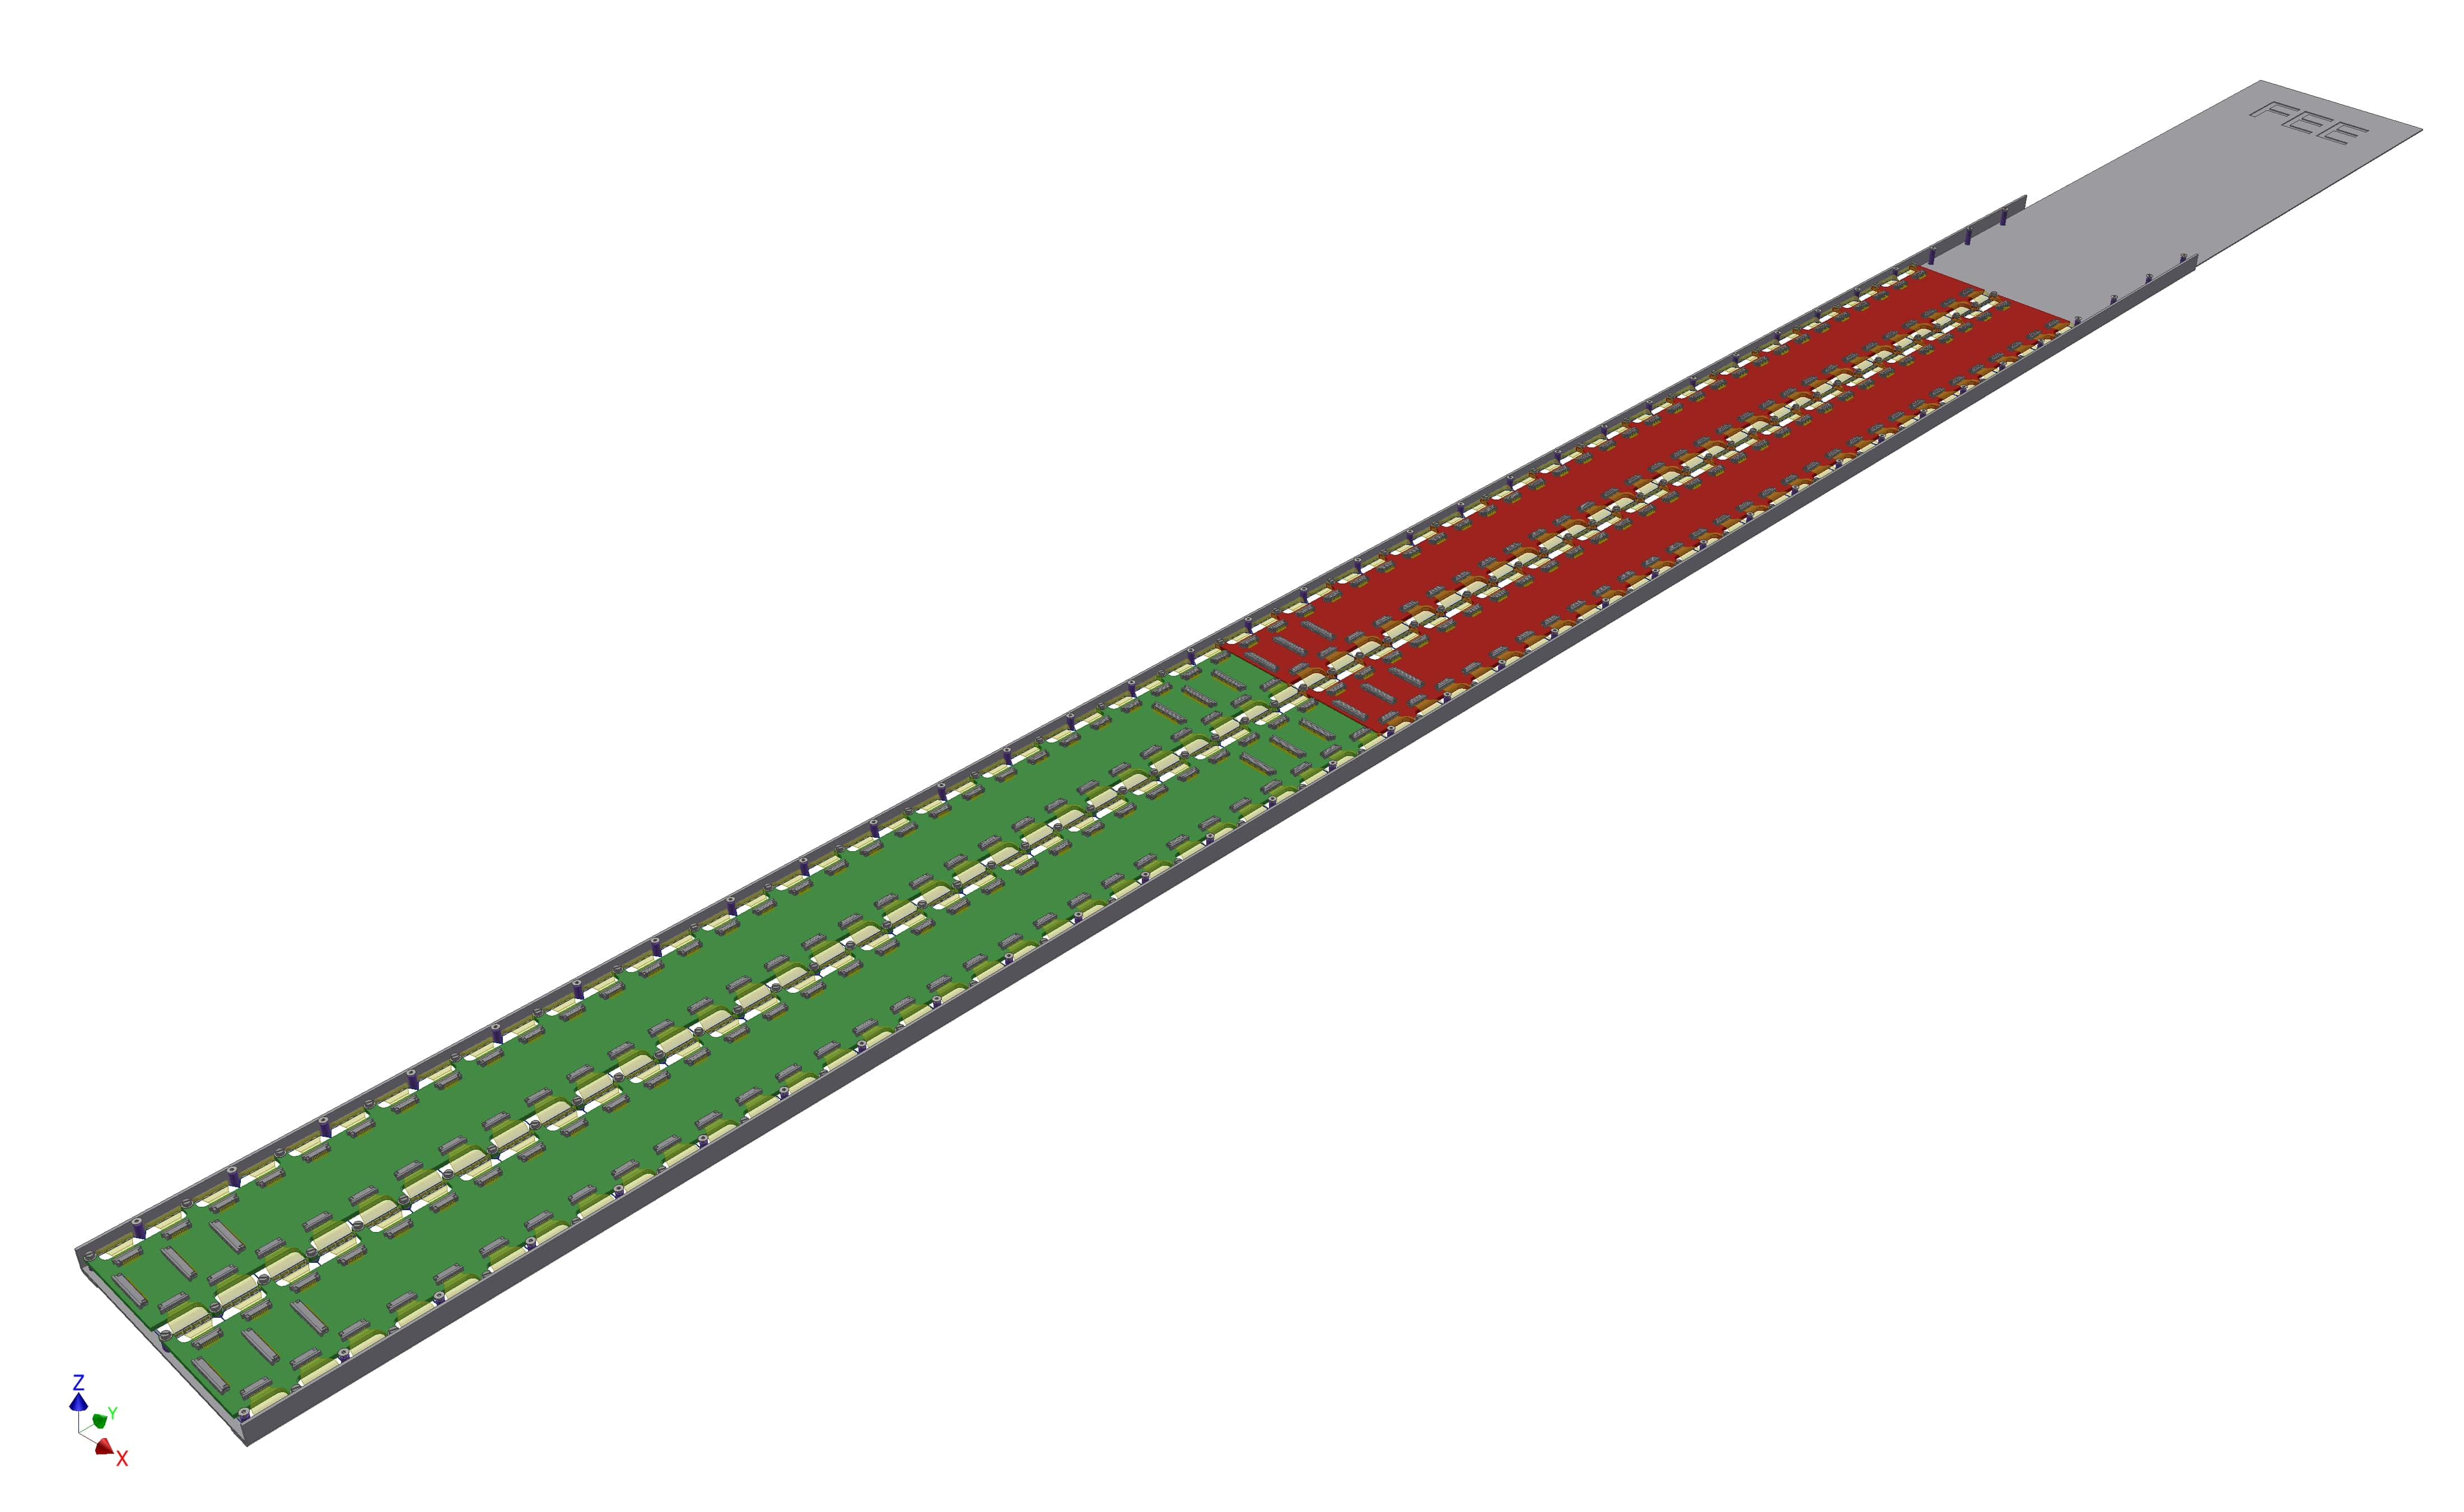
\includegraphics[width=.8\textwidth]{fig/Supermodule_Design_full_open-min.jpg}
	\caption{Full \sm\ without the FEE. It comprises a front \railboard\ (green), back \railboard\ (red), scintillators (white), \sensorboard s (yellow) and a carbon holding frame (gray).}
	\label{fig:SuperModule}
\end{figure}

A single large PCB or a PCB split into a front and back part connect the Front End Electronics (FEE) to the detector elements. 
Each \sm\ is equipped with 60 scintillator tiles in two rows, read out by four \sipms\ on each side of the scintillator. 
This adds up to 3840 channels with a total amount of \num{15360} deployed \sipms .
A cross section can bee seen in \fig ~

\begin{figure}[htbp]
	\centering
	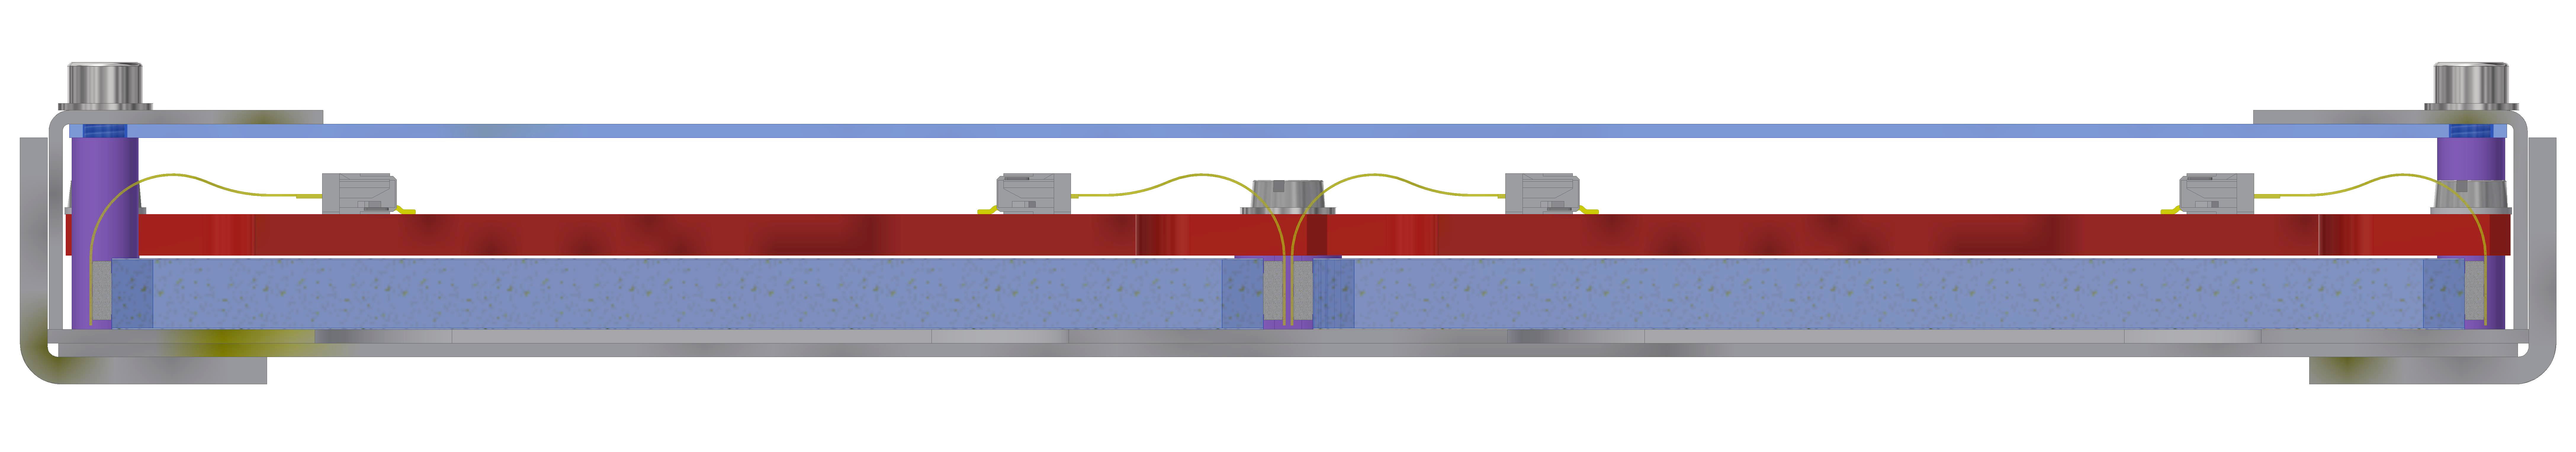
\includegraphics[width=.8\textwidth]{fig/Railboard3_Schnitt.jpg}
	\caption{Cross section of the \btof\ showing the carbon frame, the scintillators held in place by purple spacer with \sipms\ between the tiles and connected to the \railboard\ via flexible \sensorboard PCBs.}
\end{figure}

\subsection{Scintillator}
Each scintillator of the \btofD\ is identical to the others and have the following dimensions; \SI{87 x 29.4 x 5}{mm}.
To fit inside the holding structure the corners of the scintillator tiles are truncated.
Each chamfer is set at \SI{3}{mm}.
This is a change from the design proposed in the Technical Design Report (TDR) which had rectangular scintillators.

\subsubsection*{Material}
The scintillator of choice for the detector dimensions is the EJ-232 by Eljen Technology. It is an organic scintillator compound developed for high accuracy timing applications \footnote{\url{https://eljentechnology.com/products/plastic-scintillators/ej-232-ej-232q}}.
The equivalent Saint-Gobain/Bicron equivalent product would be the BC-422 scintillator.
Another material candidate was the widely used EJ-228/BC-418.
It produces more photons but for the small dimensions of the \btof\ tiles delivers a slightly inferior time resolution.
%Due to the short emission wavelength the mean free path inside of the scintillator is only around \SI{10}{cm}.

Measurements comparing the scintillator thickness revealed stark differences in performance between \SI{3}{mm} and \SI{6}{mm} thick tiles. 
Under ideal circumstances, for equal readout surface and constant energy loss of passing particles, the number of detected photons is independent of the thickness.
However, since the number of internal reflections is increased for thinner tiles, more photons are lost at the scintillator surface compared to thicker modules.
This leads to a significant time resolution increase when reducing the tile thickness as can be seen in \fig ~\ref{fig:Tchickness_timeRes}.
Since the performance difference between \SIlist[]{5;6}{mm} is minimal and the material budget of the device needs to be kept at a minimum the detector will be equipped with \SI{5}{mm} thick tiles.

\begin{figure}[htbp]
	\centering
	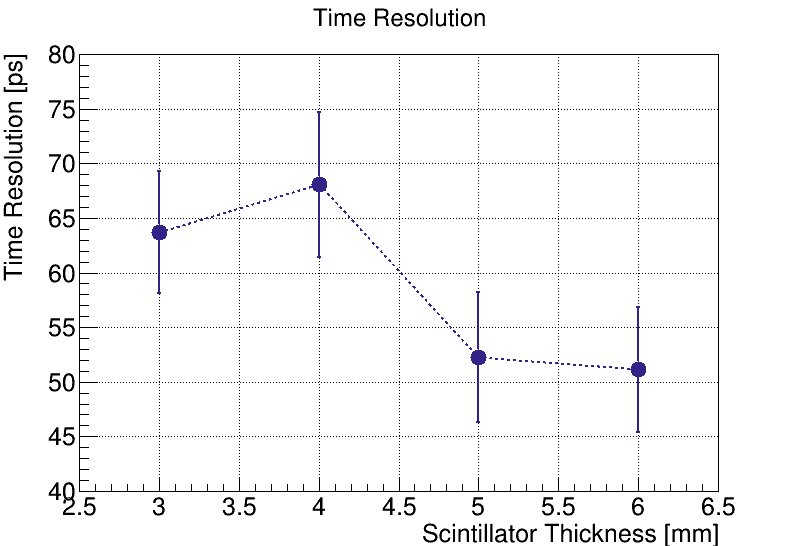
\includegraphics[width=.7\textwidth]{fig/TimeResSummary.png}
	\caption{Time resolution measurement comparing different thicknesses of aluminized mylar wrapped scintillator tiles.}
	\label{fig:Tchickness_timeRes}
\end{figure}

\subsubsection*{Wrapping}
Since the time resolution of a scintillator detector is coupled to the number of detected photons, the scintillator tiles are wrapped in order to reflect photons that escape the scintillator back into it.
The material choice was subject to tests performed on a scintillator tile using a \sr\ source in order to determine the best performing wrapping.
Material candidates were aluminized mylar foil, Tyvek hardstructure 1057D, enhanced specular reflector (ESR), Teflon tape, aluminum foil and no wrapping.
As can be seen in Table~\ref{tab:WrappingTest}, taken from the \btof\ TDR\footnote{\url{https://panda.gsi.de/system/files/user_uploads/ken.suzuki/RE-TDR-2016-003_0.pdf}}, the performance difference was within \SI{6.7}{ps} from the best to the worst performing wrapping and a standard deviation of \SI{2.23}{ps}.

\begin{table*}[htbp]
	\caption[Time resolution for different wrapping materials]{Time resolution of EJ-232 (top) and EJ-228 (bottom) plastic scintillator tiles for various wrapping materials.
		\label{tab:WrappingTest}}
	\centering
	%\resizebox{0.8\textwidth}{!}
	{
		\begin{tabular}{ l  c  c }
			\toprule
			Wrapping material                 & Time resolution [ps] & Number of detected photons \\
			\midrule
			No wrapping                       & 55.0\,$\pm$\,0.3     & 288\,$\pm$\,2\\
			Aluminized Mylar foil             & 52.7\,$\pm$\,0.3     & 355\,$\pm$\,2\\
			Tyvek hardstructure 1057D         & 55.0\,$\pm$\,0.3     & 394\,$\pm$\,3\\
			Enhanced specular reflector (ESR) & 55.2\,$\pm$\,0.3     & 355\,$\pm$\,3\\
			Teflon tape                       & 59.4\,$\pm$\,0.3     & 408\,$\pm$\,4\\
			Aluminum foil                     & 54.2\,$\pm$\,0.3     & 344\,$\pm$\,3\\
			\midrule
		\end{tabular}
	}
\end{table*}

Surprisingly, Teflon tape, the by far worst performing wrapping, produced the largest amount of detected photons.
The best performing material and the only one better than no wrapping at all was the aluminized mylar foil.
This can be attributed to the type of reflection.
While aluminized mylar has a mirror like finish, the other materials produce diffuse reflections.
This leads to larger distances travelled by the photons before reaching the photo detectors.

The wrapping material of choice for the scintillator tile of the \btofD\ is aluminized mylar.


\subsection{\sipm}

To detect the photons produced in the scintillators a device is needed that fits into the limited space available to the detector, can operate within a strong magnetic field and delivers a good time resolution.
A sensor that fits these criteria is the Silicon Photomultiplier (\sipm ).
These small devices are available in multiple sizes.
Best suited for the \btofD\ is an effective photosensitive area of \SI{3x3}{mm} with a thickness in the order of \SI{1.5}{mm}.

Multiple manufacturers offer sensors of such kind including \hamamatsu, \ketek and \advansid\ each with slightly different operational parameters.
One main point to consider is the operational voltage which differs greatly between manufacturers.
While \hamamatsu\ \sipms\ are operated at around \SI{60}{V}, \ketek\ \sipms\ only require a bias voltage of around \SI{30}{V}.
Since the sensors will be connected in series as described in Section 4.2 of the \btof\ TDR, the operational voltage is 4 times the single sensor voltage, which affects the requirements from necessary electronics to drive the sensors.

The final choice on which \sipm\ model to use has not been made since the development of \sipms\ moves relatively fast and new product generations were expected.
Tested sensors include the \texttt{S13360-3050PE} by \hamamatsu, the \texttt{PM3350} by \ketek\ and the \texttt{ASD-NUV3S-P} by \advansid , which all perform adequately.

\subsubsection*{Serial connection of 4 \sipms}

In order to effectively readout the \SI{5x30}{mm} large surface area of the ends of the scintillator tile, the active surface needs to be extended beyond a single \sipm\ with an effective photosensitive are of \SI{3x3}{mm}.
To do this four \sipms\ are connected in series.
This offers a larger active area without increasing the detector complexity by adding unnecessary channels by reading out the \sipms\ individually.

Additionally connecting the sensors in series in contrast to a parallel connection, offers an improvement of the signal timing properties.
The slope of the rising signal flank, which determines the signals timing susceptibility to electrical noise, depends on the sensors internal capacitance.
A smaller capacitance leads to a faster sensor discharge and a steeper signal slope.
Connecting the sensors in series decreases this internal capacitance making the signal faster whereas a parallel connection would have the opposite effect.

There is evidence suggesting, that increasing the amount of \sipms\ from 4 to 6 would improve the time resolution.
These tests however were performed at a time where the scintillator was held in place differently and hence was not chamfered.
Cutting away \SI{3}{mm} from either edge reduces the available space to \SI{24}{mm}.
With the actual width of each \sipm\ is slightly below \SI{4}{mm} and an LED between the middle two sensors, there simply is not enough room for additional sensors.

\subsection{\sensorboard}

To connect the \sipms\ to the readout they are soldered onto a flex PCB called the \sensorboard .
It not only holds the photon sensors but also the temperature sensor and a calibration LED.
To establish a secure connection between the \sipms\ and the scintillator it is glued onto the scintillator tile as seen in \fig~\ref{fig:SensorBoradNew}.

\begin{figure}[htbp]
	\centering
	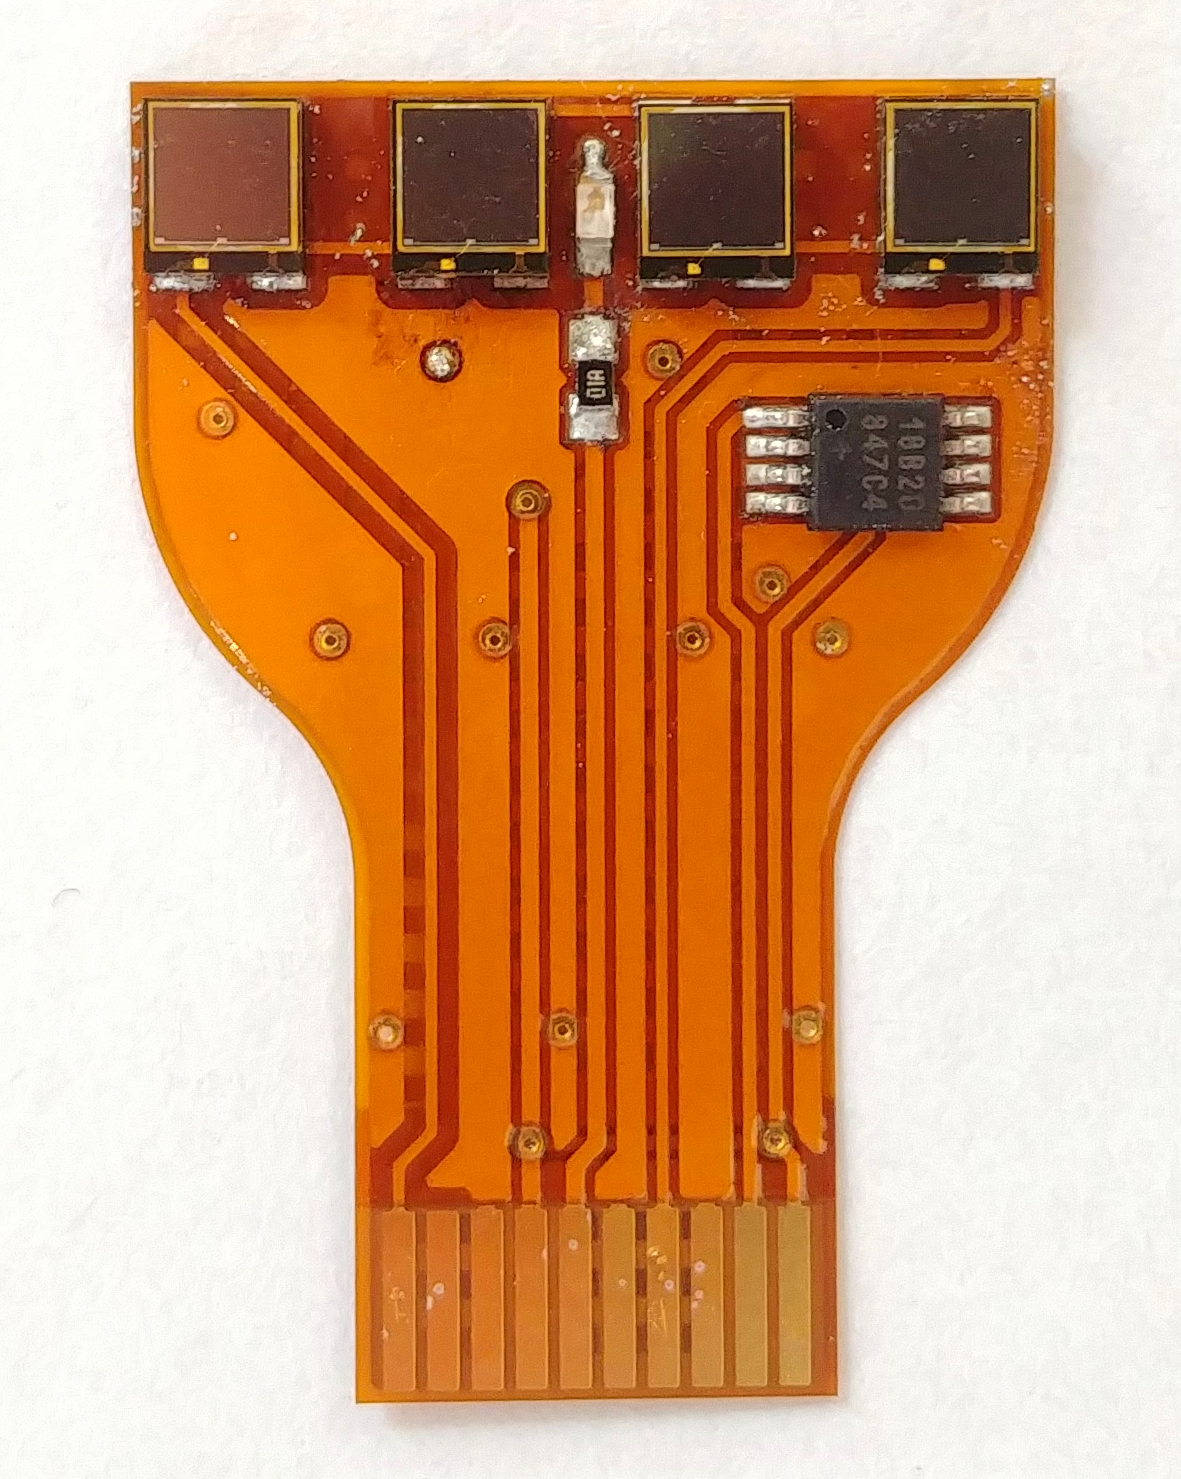
\includegraphics[height=5cm]{fig/SensorBoardNew2.png}
	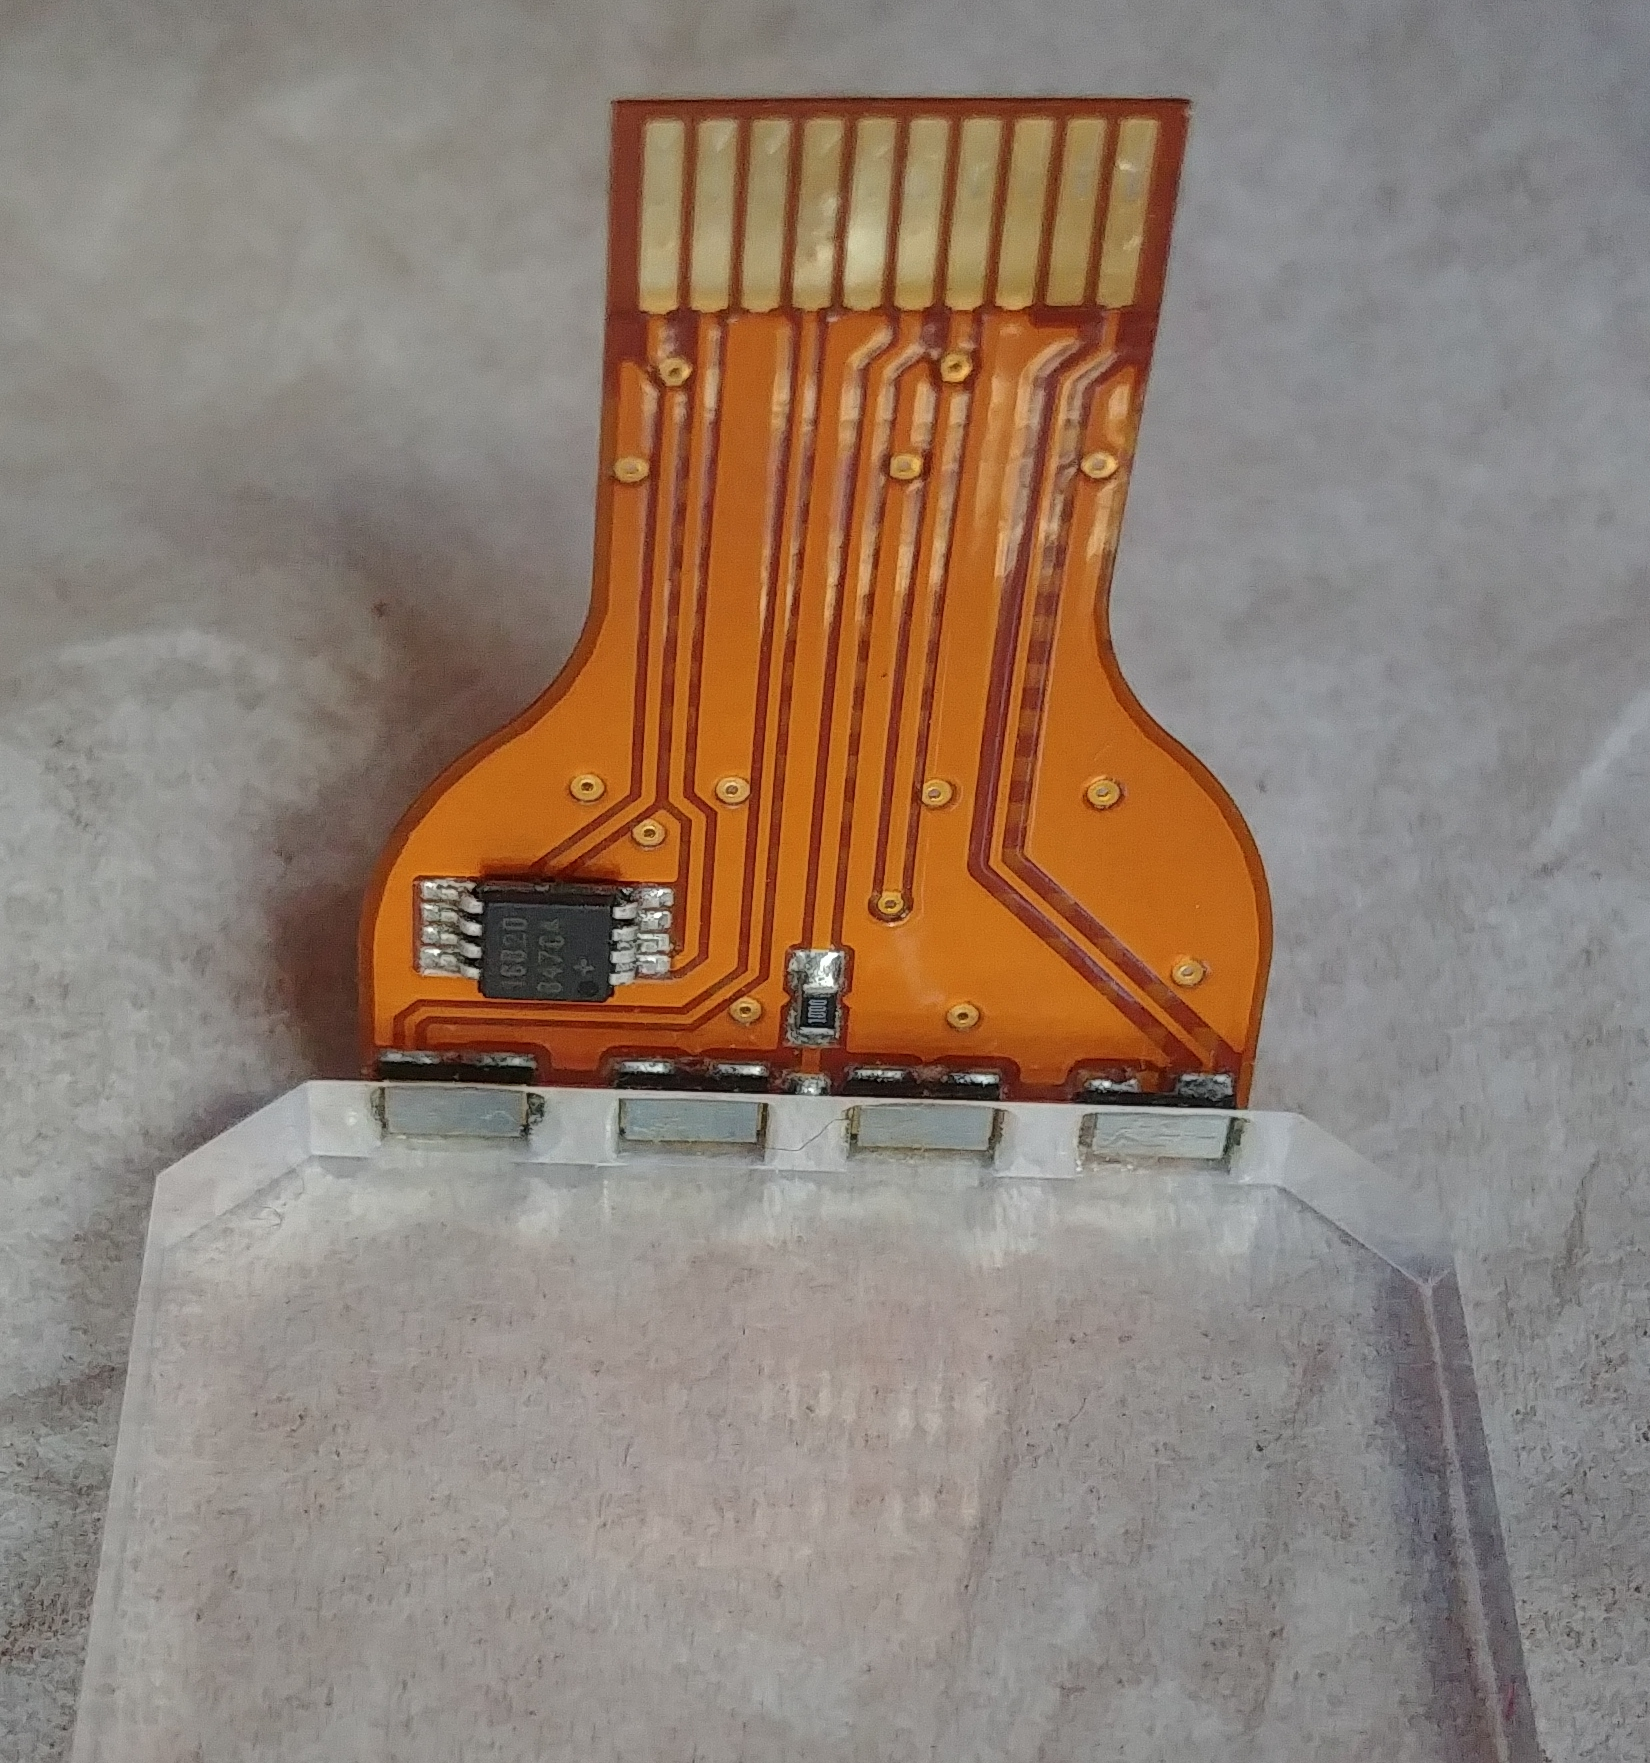
\includegraphics[height=5cm]{fig/Sensorboards2Scintillator.jpg}
	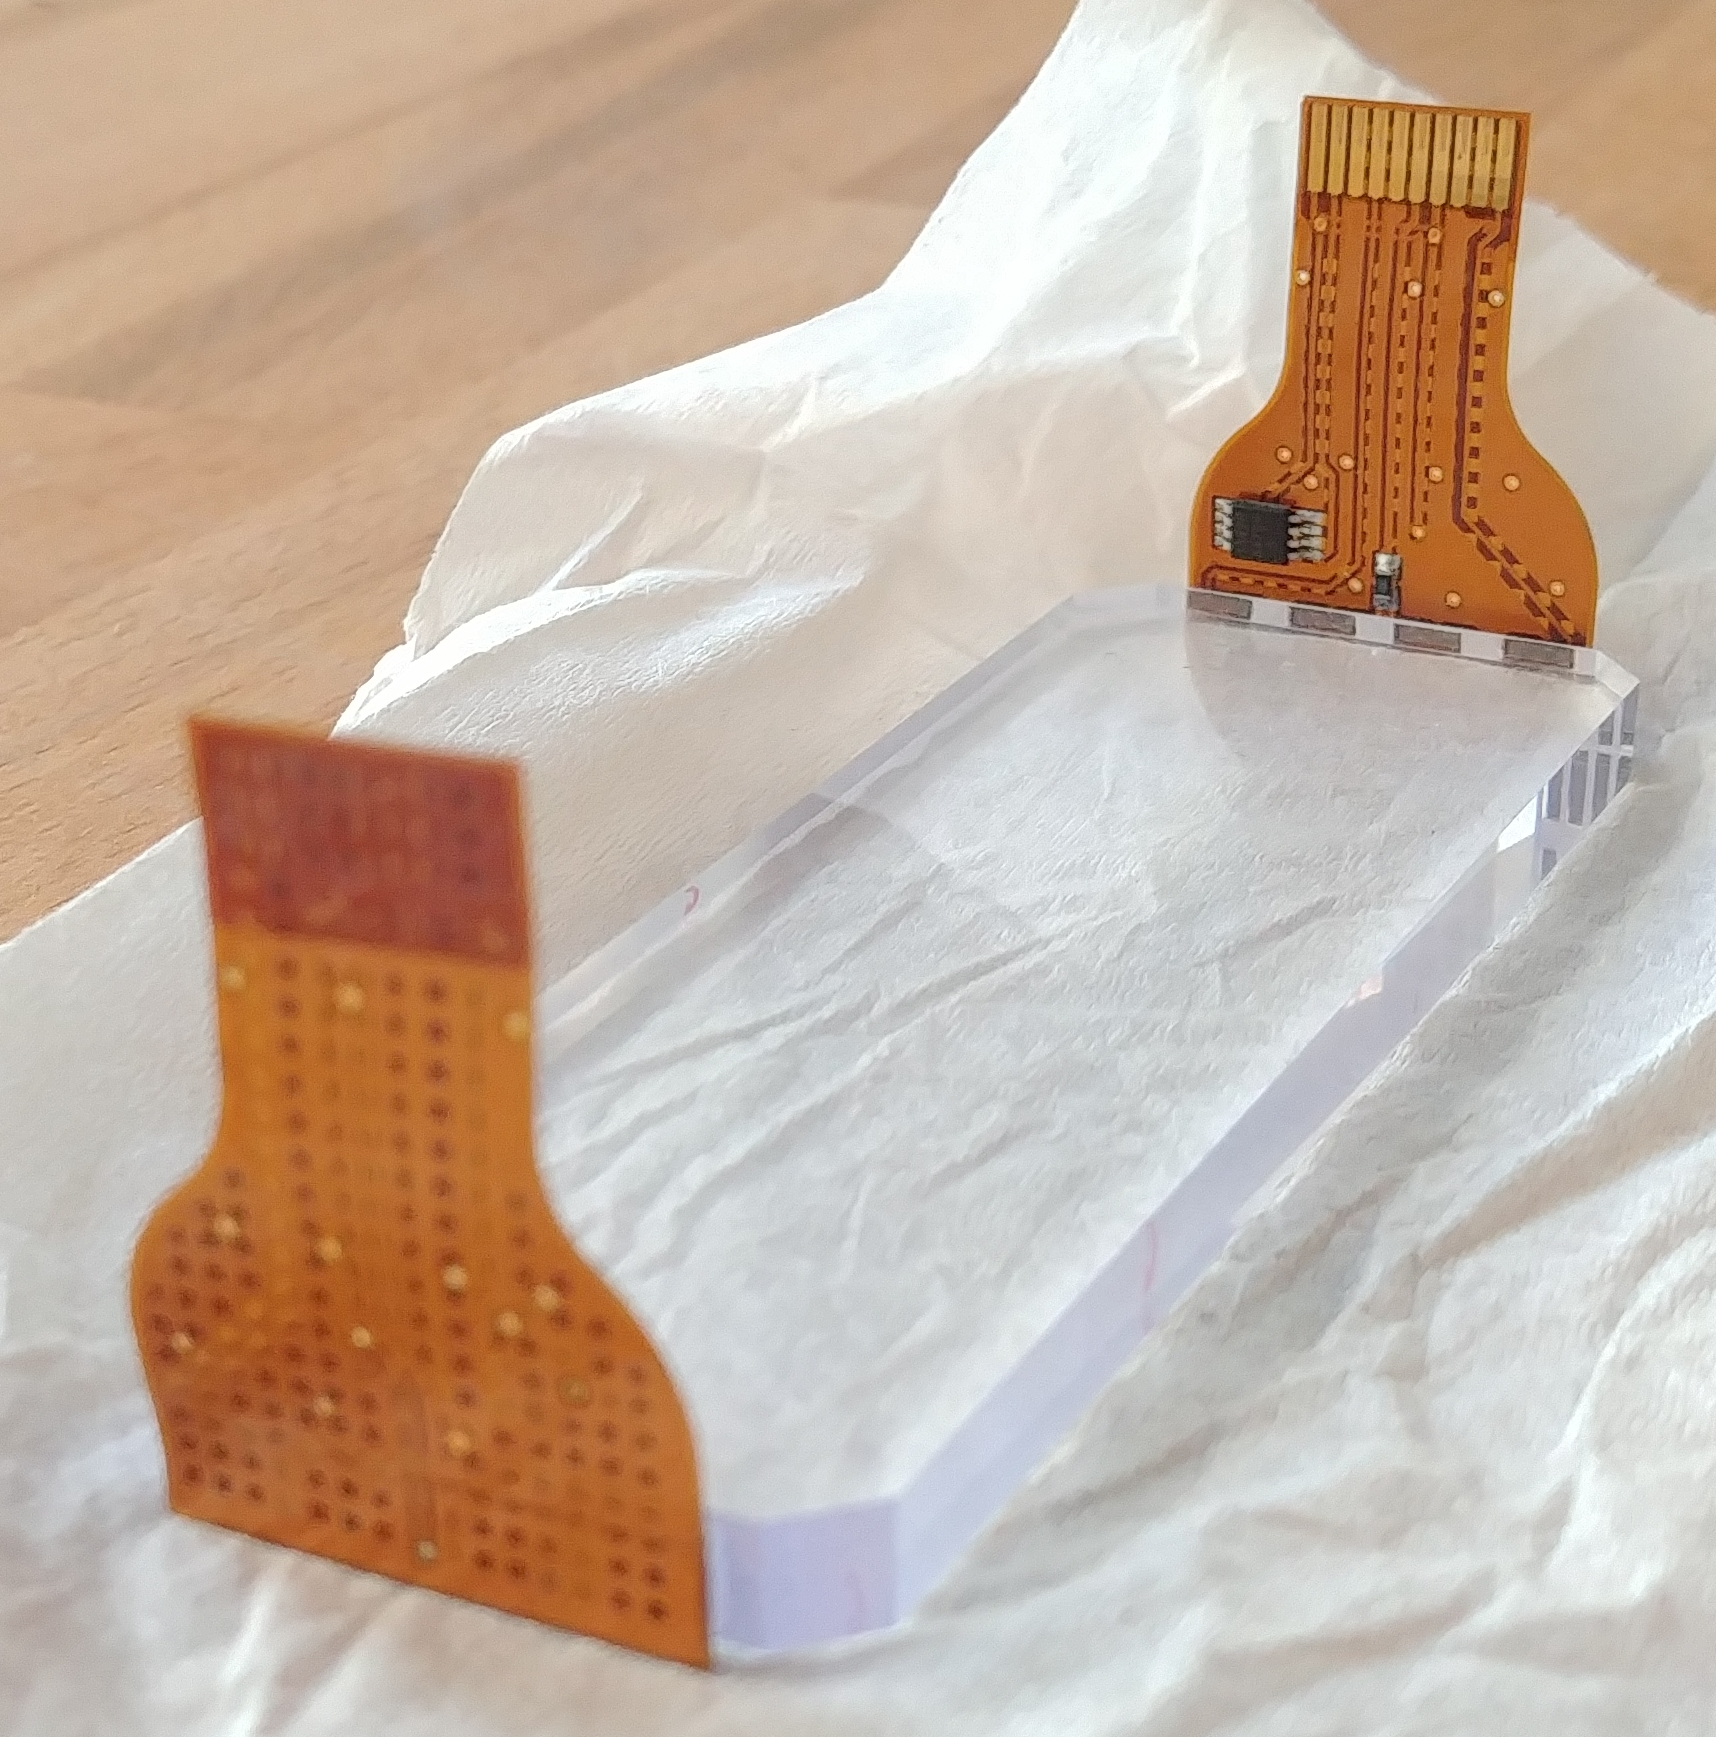
\includegraphics[height=5cm]{fig/Sensorboards2Scintillator2.jpg}
	\caption[The flexible \sensorboard .]{A flexible \sensorboard\ featuring four \sipms\ in series, a temperature sensor and an LED (left), attached to a scintillator (middle) and a full active module (right).}
	\label{fig:SensorBoradNew}
\end{figure}

To ensure a matching characteristic impedance the line dimensions need to be controlled.
A possible layout to achieve a characteristic impedance of \SI{50}{\ohm} would be a flex board from \texttt{beta-layout.com} who produce flexible embedded microstrip boards with a subtrate thickness of \SI{80}{\micro m} with \SI{50}{\micro m} of cover film, a copper strength of \SI{18}{\micro m} and a dielectric constant of 3.2 to 3.3.
With a line width of \SI{257}{\micro m} this produces an impedance of \SI{49.94}{\ohm}.

Our first version of these boards however were not properly impedance matched.\todo[]{what are the dimensions of the first boards?}

Important findings during the testing of this new board is that the thin copper lines are very fragile.
Multiple strong bends can sever the connection between the \sipms\ and the \railboard .
For this reason it is important to handle these boards with care.
To remedy this the transition of the \sipm\ solder pad to the transmission line was changed from a strict \ang{90} corner to a smoother teardrop shaped junction.\todosvetlana[]{add info on how this change affected the reliability of the boards}
\todo[inline]{the first version of these boards whas not propperly impedance matched. The second version should be by increasing transmission line width and adding a copper back plane.}

\subsubsection*{Calibration LED}
The LED is supposed to function as a calibration and monitoring device during the operation of the detector.
Calibrated signals are produced by flashing the LED.
Long term changes in amplitude or time resolution can be picked up and monitored, catching the eventual progression of the detector deterioration.
The development of this procedure was subject of the work of a masters student who however never finished.
Since then the technique past the first idea has not been further developed.

It would be necessary to determine the best way to drive the LEDs in order to produce a short and well defined signal. 
This includes the optimal voltage and duration of the driving signal, as well as determining what LED specifically would be optimal.
In general it is best to keep the emitted wavelengths as close to the scintillator light as possible to monitor the relevant performance.
Ultimately this development would need to be made in combination with finalizing the electronics of the whole system.

%%%%%%%%%%%%%%%%%%%%%%%%%%%%%%%%%%%%%%%%%%%%%%%%%%%%%%%%%%%%%%%%%%
\subsubsection*{Temperature Sensor}
In order to monitor the climate the scintillator tiles and the \sipms\ are subject to, every sensor board is equipped with a temperature sensor. It was important that these devices can be read out using a minimal amount of channels or transmission lines to keep the material budget and \railboard\ occupancy at a minimum.
Individual channels for all 240 \sensorboard s per \sm\ would also overload the readout system.

A solution to this is a digital temperature sensor on a 1-Wire bus.
This bus offers the capability to connect a large amount of sensors in parallel, only requiring a ground, signal and power supply line.
Such a sensor is the \texttt{DS18B20} by \textit{Maxim Integrated}.
These sensors can be controlled by a micro controller and utilize a hard coded 48-bit address for each sensor, which far exceeds the number of necessary sensors for one \railboard .
To power them a bias voltage between \SIrange[]{3}{5.5}{V} is required.
A schematic of the connection of such sensors can be seen in \fig ~\ref{fig:DS18B20_connection}.
It is the sensor used in the prototype.
It has been tested separately but not yet on the \railboard .

\begin{figure}[htbp]
	\centering
	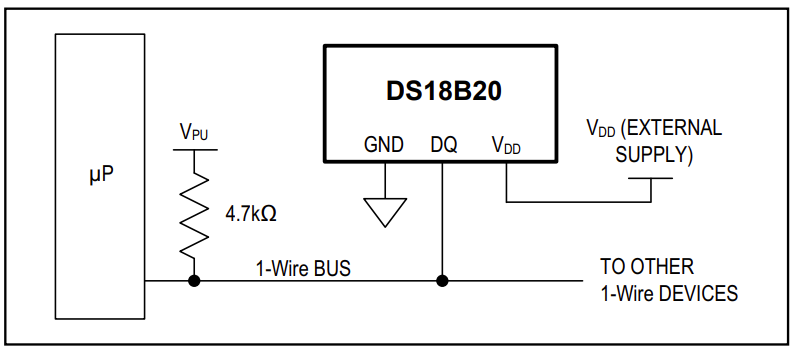
\includegraphics[width=.6\textwidth]{fig/DS18B20_connection.png}
	\caption[Connection scheme for the DS18B20 temperature sensor.]{Connection scheme for the DS18B20 temperature sensor connected to a micro processor (µP).}
	\label{fig:DS18B20_connection}
\end{figure}

The readout process consists of two parts, the initial command to measure the temperature and write the value into memory and secondly the process of retrieving this information.
Together this can take up to \SI{1.5}{s} for 60 sensors.
Every additional sensor would require an addition \SI{12}{ms}.
This means that for all 240 sensors on one \sm\ the readout would take up to \SI{3.8}{s}.
With signal amplitudes between \SIlist{3.3;5}{V} the resulting crosstalk prevents any meaningful data taking in this time.


\subsection{\railboard}

The solution to connect the photo sensors to the FEE and provide mechanical support at the same time is the \railboard .
It is a long PCB split into two parts due to availability issues of the base material.

Previous designs relied solely on the mechanical support of a single \railboard\ spanning the entirety of a \sm\ to hold all components including the scintillators in place.
Due to stability issues and too small tolerances in the connectors the connection scheme and with it the form of the board has been redesigned and a carbon frame has been added.
The single \railboard\ is replaced by four large PCB's, one of which is shown in \fig ~\ref{fig:Railboard}.
Two of these boards are attached by ribbon cables to connect one full row of 60 scintillators to the FEE and held in place by plastic screws to the carbon frame.

\begin{figure}[htbp]
	\centering
	\includegraphics*[width=.9\textwidth]{fig/Railboard3_imageCombined.png}
	\caption{Combined depiction of the internal transmission line layout and a photograph of the front part of the \railboard .}
	\label{fig:Railboard}
\end{figure}

Each board consists of 16 conductor layers alternating between shielding ground layers, which span the almost the entire layer and signal transmission lines, which can be seen in \fig ~\ref{fig:Railboard3_schematic}.
Since resistive losses at the relevant frequencies are dominated by the skin effect it is necessary to keep the conductor surface as large as possible.
In order to maximize the conductor surface while minimizing the material budget all conductor layers are kept as thin as possible with a thickness of \SI{17}{\micro \meter}.
For the purposes of minimizing reflection losses, the characteristic impedance of the whole board was kept around \SI{50}{\ohm}.
For this the relation between the width of the transmission lines and the substrate thickness had be calculated.
Since vertical space is limited a laminate thickness of \SI{0.406}{mm} was chosen which mandates a transmission line width of \SI{400}{\micro m}.

\begin{figure}[htbp]
	\centering
	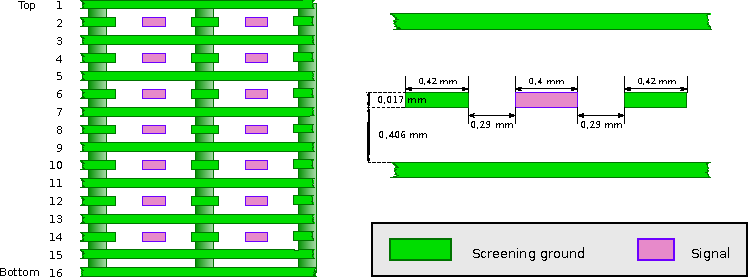
\includegraphics[width=.9\textwidth]{fig/Railboard3_schematic.pdf}
	\caption{Schematic of the internal layout of the \railboard\ conductors. The board substrate material RO4003C is left blank.}
	\label{fig:Railboard3_schematic}
\end{figure}

% low loss material
\sipm\ signals with a rise time of \SI{3}{ns} correspond to a frequency of \SI{167}{MHz}.
At this frequency dielectric losses start to take on a larger portion of the electric losses experienced along a transmission line as seen in \fig~\ref{fig:LowLossCurve} \footnote{more information in the dissertation "Development of the Fast Timing \panda\ Barrel Time-of-Flight Detector" by S. Zimmermann}.
To reduce these losses special PCB substrate materials have been developed such as RO4003C by Rogers Corp.
This is the material that is used for the \btof\ \railboard\ to ensure minimal losses for an optimal performance.

\begin{figure}
	\centering
	\includegraphics*[width=.8\textwidth]{fig/Loss_Curve_Sebastian_v3.pdf}
	\caption{Simulation of the resistive and dielectric losses expected for a \SI{400}{\micro m} wide \SI{50}{\ohm} impedance stripline in FR-4.}
	\label{fig:LowLossCurve}
\end{figure}

\subsubsection{\railboard\ Split}

The \railboard\ was split out of necessity to be able to use the chosen low loss material, which was initially meant to decrease the signal attenuation along the board.
Since RO4003C sheets are not available beyond 48 inches or \SI{1.224}{m} the boards need to be split into a front and back part each holding 30 scintillators.
The mentioned size is the standard sheet size.
We did not make inquiries to determine whether larger nonstandard sizes were available.
Boards made out of FR-4 however are available in large sizes although few companies are able to handle such boards sizes.
Companies such as Thales in the Netherlands or Micro-Pattern Technologies at CERN are equipped with the necessary technical facilities to be able to produce boards of sufficient size.

After further investigation, the positive influence of the low loss material on the signal amplitude is most likely negligible at the expected signal frequencies of around \SI{350}{MHz}.
The larger performance improvement from the second to the third \railboard\ generation is due to the increased width.
The larger benefit of using Rogers Material is the material budget savings it provides.
Due to its smaller dielectric constant the distance and the amount of material between layers in the \railboard\ is reduced compared to regular FR-4, in order to keep the characteristic impedance of \SI{50}{\ohm}.

The drawback of the split however is that a connection between the boards needs to be established which potentially introduces unwanted behavior by picking up noise or introducing losses when not perfectly impedance matched.
It needs to evaluated if the gains from using Rogers Material outweigh the drawbacks of splitting the boards.

Since the board is split already and requires external support it only makes sense to separate the scintillator rows along the long axis.
This gives the detector a higher degree of modularity and makes installation and swapping of components easier.

%%%%%%%%%%%%%%%%%%%%%%%%%%%%%%%%%%%%%%%%%%%%%%%%%%%%%%%%%%%%%%%%%%%%%%%%%%%%
\subsection{Connectors and Connections}

The board is equipped with three types of connectors, that 
\begin{enumerate*}[label=\textbf{\Roman*})]
	\item  connect the two halves of the \railboard\ to one another, 
	\item the \sensorboard s to the \railboard\ and 
	\item establishes a connection between the \railboard\ and the TOFPET ASIC.
\end{enumerate*}

\textbf{I)} 
The boards are connected by ribbon cables.
The design of these cables has not been studied or optimized.
They should optimally possess a characteristic impedance of \SI{50}{\ohm}.
The cables used for the prototype do not quite fulfill that requirement.
Each transmission line meant for \sipm\ signals is \SI{0.9999}{mm} wide with a separation of \SI{0.9999}{mm} between lines.\todo[]{add true dimensions}
The lines on the cable alternate between transmission lines connected to \sipms\ and ground lines in order to reduce crosstalk between the channels.
This however limits the width of each line in order to fit them all in the \SI{4}{cm} wide cable.\todo[]{add true width}
To improve the transmission properties a copper back plane is added to the ribbon cable effectively making it a two layered board.
One possible improvement would be to reduce the width or take out a number of the ground lanes to free up space.
This is possible since the crosstalk was shown to be a nonissue.
Additionally the prototype cables were both \SI{20}{cm} long.
This gives the prototype some flexibility during the design phase.
For the final design the cables should be shortened to the respective distance between the connectors.
This makes one cable longer than the other.

The connectors for the ribbon cables between the boards as well as the connectors for the \sensorboard s are FFC/FPC\footnote{Flex Flat Cable / Flex Printed Circuit} connectors.
To connect the two \railboard\ halves, as shown in \fig ~\ref{fig:Railboard_connection} two distinct FFC connectors are used.
Transmission lines which carry detector signals are connected via the \texttt{FH28-60S-0.5SH} connector by Hirose Electric Group, which is depicted in \fig~\ref{fig:Railboard_connector}.
These connectors are only rated up to \SI{50}{\ohm} but since only event signal pulses travel down this line this is sufficient.

Connections for the power delivery and the temperature sensors are connected using the \texttt{ZF1-25-01-T-WT-TR} by Samtec, shown in \fig~\ref{fig:Railboard_power_connection}.
These connectors are rated up to \SI{215}{V} of working voltage and a break down voltage of \SI{875}{V}.

The main difference between the two connectors is the pitch size of connectors pins.
Since there are many more signal lines on the \railboard\ than power lines, these have higher pitched connectors.
If the number of power lines is to be increased this could be changed.
It however is important to keep in mind that the higher the pitch of the connector, the closer each line is to one another physically limiting the voltage it can successfully sustain.

\begin{figure}[htbp]
	\centering
	\includegraphics[width=.7\textwidth]{fig/Railboard_Connection_filter.png}
	\caption{Connection between the \railboard\ halves.}
	\label{fig:Railboard_connection}
\end{figure}

\begin{figure}[htbp]
	\centering
	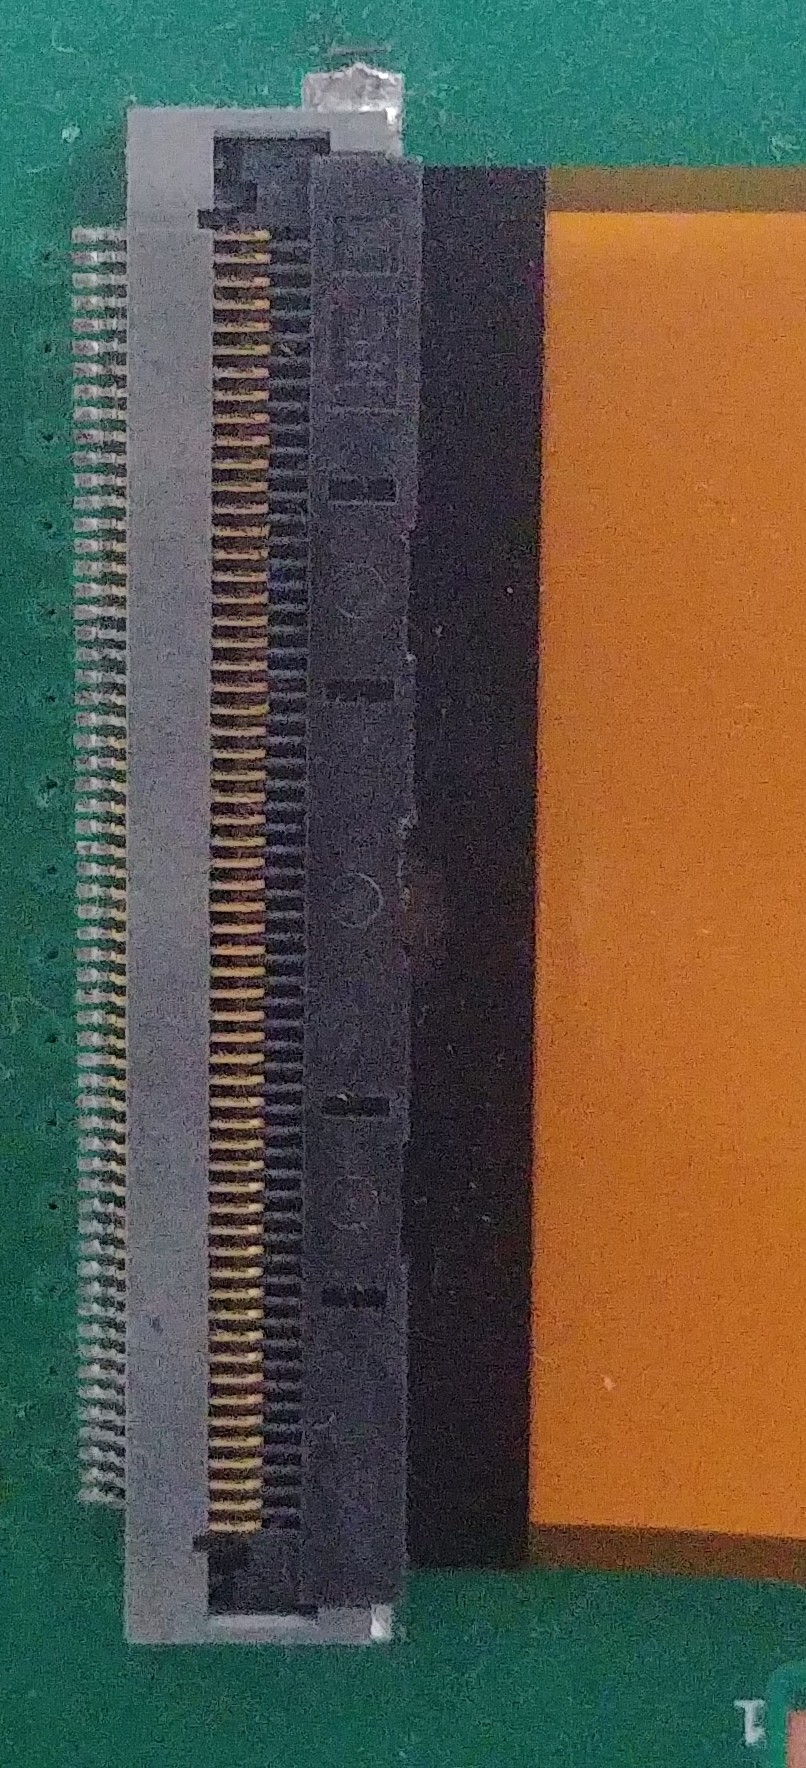
\includegraphics[height=5cm]{fig/LargeConnector_cable_crop.jpg}
	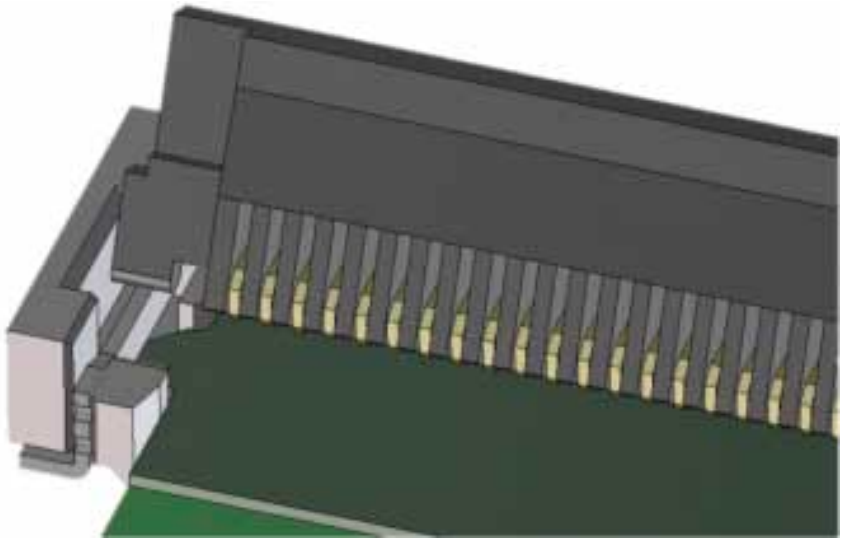
\includegraphics[height=5cm]{fig/hirose_connector_drawing.png}
	\caption{Foto and drawing of the \railboard\ connector for the ribbon cable between boards.}
	\label{fig:Railboard_connector}
\end{figure}

\begin{figure}[htbp]
	\centering
	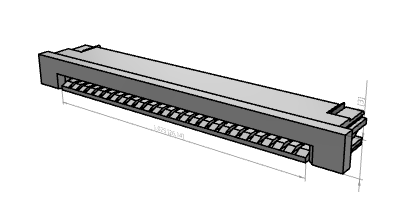
\includegraphics[height=5cm]{fig/Connector_ZF1-25-01.png}
	\caption{Connector for power and LED signals between \railboard s.}
	\label{fig:Railboard_power_connection}
\end{figure}

\textbf{II)} Similar connectors are used for the \sensorboard s, which are also connected via flat ribbon cable connectors.
The model used is a zero insertion force connector by Samtec (\texttt{ZF1-10-01-T-WT-TR}) depicted in \fig~\ref{fig:SensorBoard_connector} with a naked \sensorboard .
It is the same type of connector as above only with a reduced number of channels.
To open the connector the black plastic tab is pulled out.
After the \sensorboard\ is inserted or extracted the black tab is pushed closed to fasten the board inside and establish a secure connection.
\todo[inline]{add more info on the connectors.}

\begin{figure}[htbp]
	\centering
	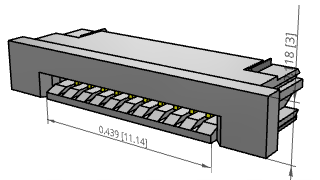
\includegraphics[height=4cm]{fig/SensorBoard_connector_drawing.png}
	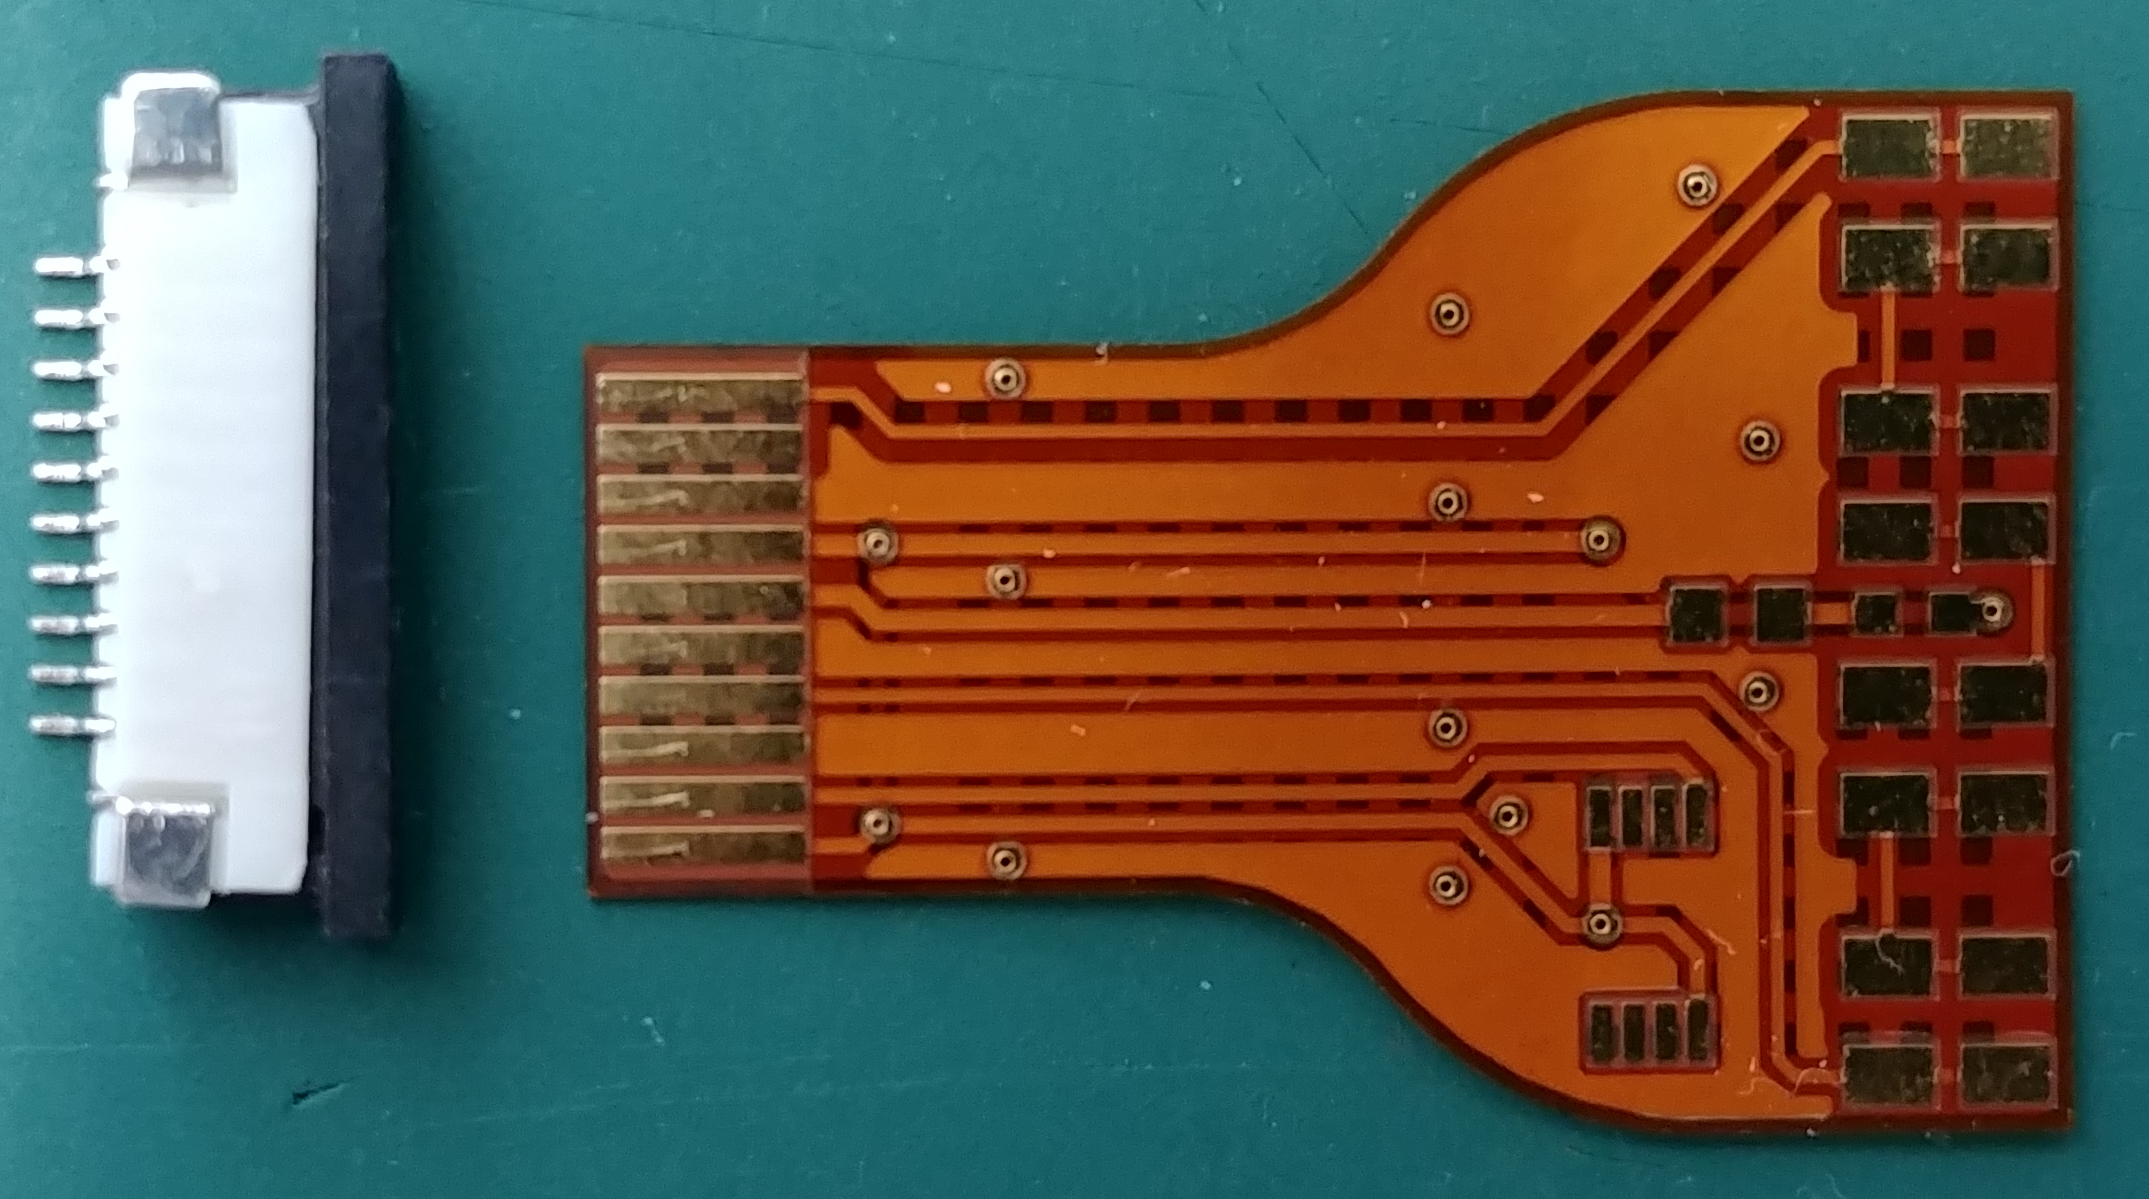
\includegraphics[height=4cm]{fig/SensorBoard_connector.png}
	\caption{Zero insertion force connector by Samtec used to connect the depicted \sensorboard\ to the \railboard .}
	\label{fig:SensorBoard_connector}
\end{figure}

\textbf{III)} The connection to the FEE has not been decided on yet since the FEE itself is not final.
The concept however is to use the connectors the PETsys boards use natively to attach them to the \railboard\ directly.
In the mean time small \texttt{MMCX} connectors are being used to quickly attach an oscilloscope or other devices such as preamps to the transmission lines.
These fasten using a simple lock-snap mechanism allowing the connected cables to be rotated freely while providing a connector with a characteristic impedance of \SI{50}{\ohm} in a minimal package.
An image showing most of these connectors soldered onto one board is shown in \fig ~\ref{fig:MMCX_connectors}.

\begin{figure}[htbp]
	\centering
	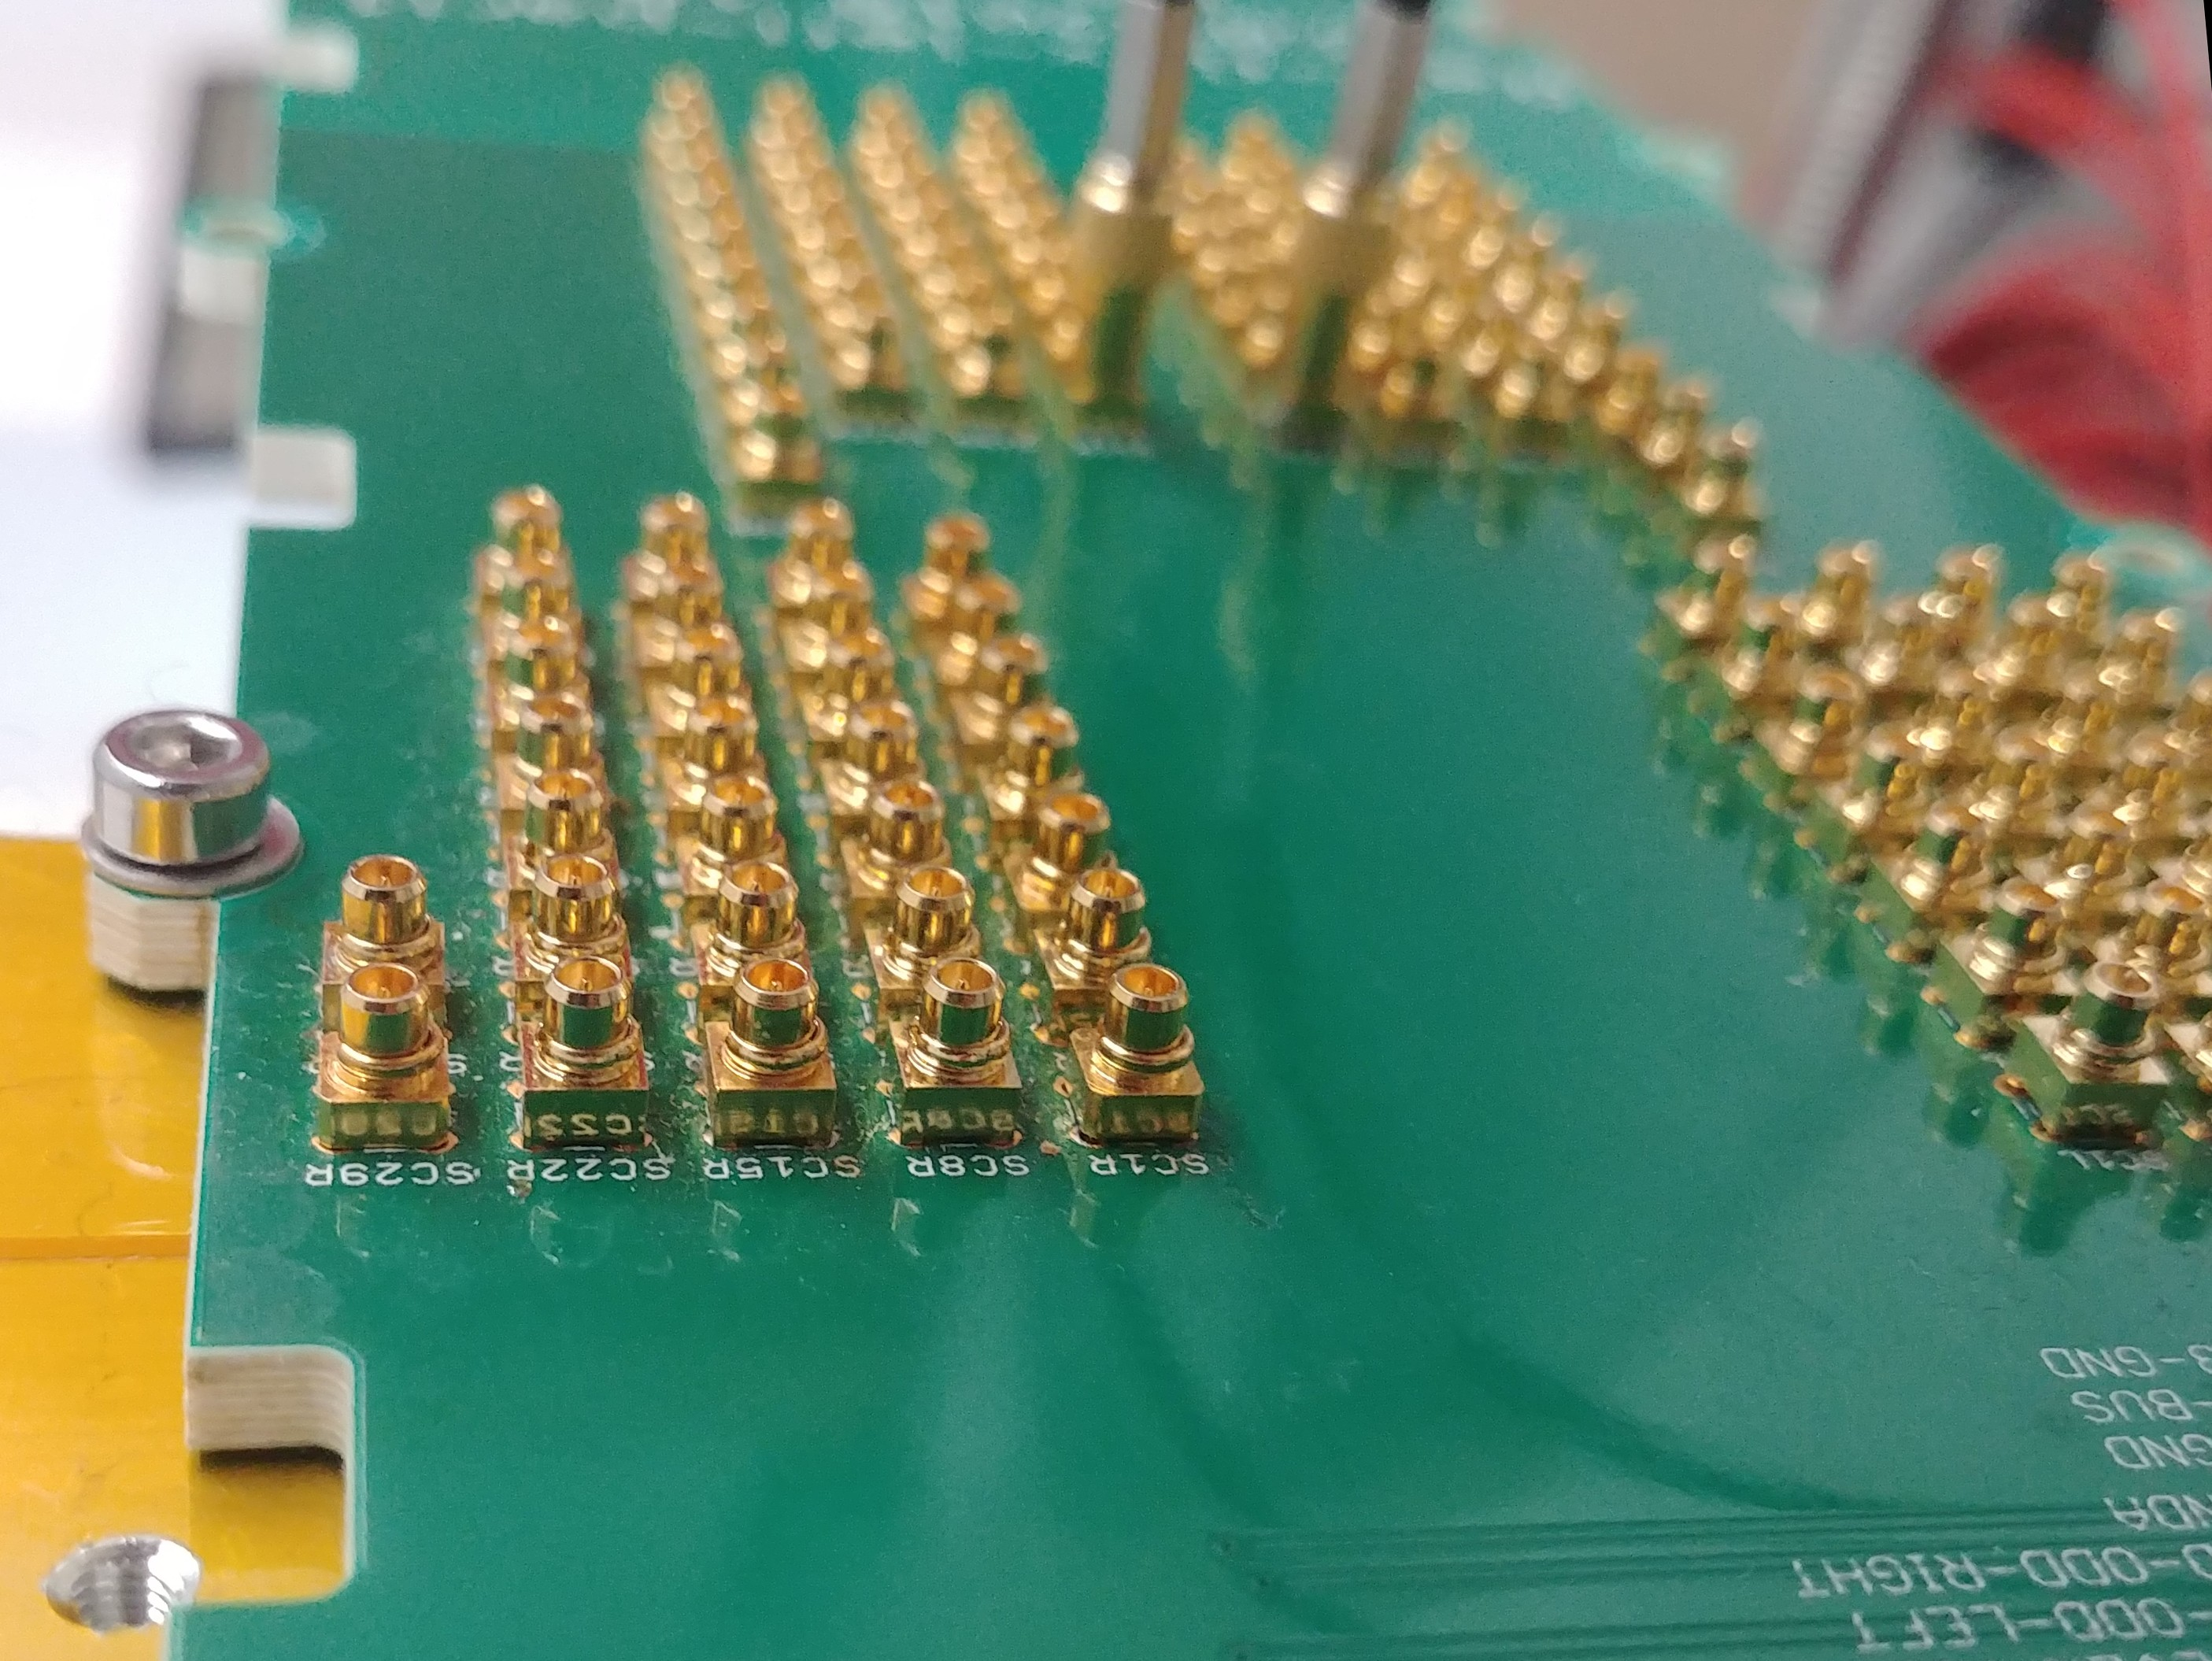
\includegraphics[width=.7\textwidth]{fig/MMCX_crop.jpg}
	\caption{All \texttt{MMCX} connectors on one \railboard\ to connect to all 120 channels with two cables connected in the background.}
	\label{fig:MMCX_connectors}
\end{figure}


%%%%%%%%%%%%%%%%%%%%%%%%%%%%%%%%%%%%%%%%%%%%%%%%%%%%%%%%%%%%%%%%%%%%
\subsection{Material Budget}
\label{sec:MaterialBudgetDesign}

In order to affect the calorimeter performance as little as possible the of material in the \btof\ has to be minimized.
The impact of the introduced material is measured in radiation lengths $X_0$.

Although it is possible to calculate an estimation of the radiation length of a certain material, it is advised to use tables of measured radiation lengths.%~\cite{gupta2010calculation}.
The data for the materials used here is provided by the Particle Data Group.%~\cite{PDG_materialData}.

To obtain the radiation length of composite materials one must add the contributions of the individual components as in Equation~\eqref{eq:Material_Budget_Sum} weighted by the components thickness ($d_i$) or mass.%~\cite{patrignani2016review}.
\begin{align}\label{eq:Material_Budget_Sum}
	\frac{d_0}{X_0} = \sum_i \frac{d_i}{X_i}
\end{align}
Since the detector does not consist of homogeneous layers the individual components must be reduced to their effective thickness spread out over the surface of the detector.

\subsubsection*{Radiation Length Estimation of Rogers Material}

Since the Rogers Material is not such a widely used PCB substrate material no information on its radiation length is available.
The only information supplied by the Rogers Corporation was that it is a hydro carbon based material filled with a ceramic (most likely Al$_2$O$_3$) and reinforced by glass fibers and provided the image shown in Figure with no further explanation. 
From the image and density information of the relevant materials one can roughly estimate the composition and its radiation length. 

\begin{figure}[htbp]
	\centering
	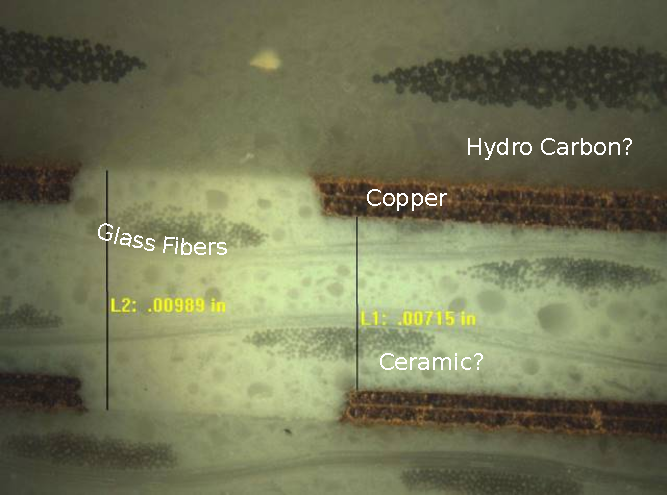
\includegraphics[width=.6\textwidth]{fig/RogersCrossSection.pdf}
	\caption[Image of the cross section of a sheet of Rogers Material RO4003C.]{Image of the cross section of a sheet of Rogers Material RO4003C, showing copper conductors surrounded by layers of a hydrocarbon substrate, filled with a ceramic (Al$_2$O$_3$) and reinforced with glass fibers.}
	\label{fig:RogersCrossSection}
\end{figure}

To calculate the radiation length, information on the material composition is necessary as seen in Equation~\eqref{eq:Material_Budget_Sum}. The exact hydro carbon is unknown and with it its density and radiation length. By estimating these values as well as the fraction of fiber glass in the board the material composition can be calculated.

Since the density ($\rho$) of the Rogers Material is known the other densities can be estimated. The density of an object is the sum of the density of its components weighted the fraction of the volume it occupies as described in Equation~\eqref{eq:RogersDensity}.
\begin{align}
	\rho_{RO} &= a \; \rho_\text{ceramic} + b \; \rho_\text{hc} + c \; \rho_\text{glass} \label{eq:RogersDensity} \\
	1 &= a + b + c \nonumber
\end{align}
The list of relevant parameters is shown in Table~\ref{tab:RO_RadiationLength}, with estimated values highlighted in blue.
Solid hydrocarbons tend to have a density of of around $\rho_\text{hc}=\SI{1.1\pm 0.15}{g/cm^3}$.
The fibers visible in Figure~\ref{fig:RogersCrossSection} take up roughly \SI{20}{\percent} of the visible layer. Assuming a fiber packing density $2/3$ that of tightly packed spheres means a volume occupancy of around \SI{10}{\percent}. 
The density dependent radiation length of hydrocarbons is rather stable no matter the exact composition with \SI{42 \pm 2}{g/cm^2}.
With the additional condition that the volume fractions have to add up to 1, Equation~\eqref{eq:RogersDensity} can be solved for $b = \num{0.705(26)}$ and $c = \num{0.195(26)}$ giving us the material composition.
Given the radiation length of Al$_2$O$_3$ and glass
%Moving forward under this premise the board is made up of \SI{19.5 \pm 2.6}{\percent} Al$_2$O$_3$ and \SI{70.5 \pm 2.6}{\percent} hydro carbon resulting in 
a radiation length of $X_0=\SI{180 \pm 15}{mm}$ can be calculated for the Rogers Material.

\begin{table}[htbp]
\centering
\caption[Values for the calculation of the radiation length of the PCB substrate material.]{Values for the calculation of the radiation length of the PCB substrate material RO 4003C which is drawn in red. Values in blue are estimates and values in black are provided.}
\label{tab:RO_RadiationLength}
\begin{tabular}{@{}lrrr@{}}
\toprule
\textbf{Material} & \multicolumn{1}{r}{\textbf{Composition}} & \multicolumn{1}{r}{\textbf{$\rho$[g/cm$^3$]}}    & \multicolumn{1}{r}{\textbf{$X_0$ [g/cm$^2$]}} \\ \midrule
RO4003c & \num{1.000}                                     & 1.79 & {\color[HTML]{C9211E} \textbf{\num{32.2(15)}}} \\
AL2O3   & \num{0.195(26)}                                 & 3.97 & 27.94                                          \\
Hydro Carbon      & \num{0.705(26)}                          & {\color[HTML]{2A6099} \textbf{\num{1.10(15)}}} & {\color[HTML]{2A6099} \textbf{\num{42.00(200)}}}      \\
Glass   & {\color[HTML]{2A6099} \textbf{\num{0.100(50)}}} & 2.4  & 25.66         \\
\bottomrule
\end{tabular}
\end{table}

\subsubsection*{\railboard\ Radiation Length Estimation}

The \railboard s are comprised of two main materials: copper and the board substrate which is RO4003C.
Since the amount of copper in the board compared to the board substrate itself is almost vanishingly small the entire volume of the board is presumed to be substrate with copper on top.
With a substrate thickness of \SI{0.2}{mm} per layer and 15 layers of substrate this amounts to a thickness of $\SI{0.2}{mm} \times 15 = \SI{3}{mm}$ which is slightly below the measured thickness of \todo{remeasure and add thickness value}.

The copper layers are split into ground plane ĺayers and such carrying transmission lines.
Each \sm\ requires 240 lines for the \sipm\ channels alone.
Other lines such as for the bias voltage, the LED's and the temperature sensor will not be considered.
A guard line with the same dimensions is placed in between each transmission line.
This brings the total up to $N_\text{lines} = 480 + 28\footnote{1 guard line for each rail and layer}$ outer guard lines per \sm .
The lines however do not run along the entire board hence a geometrical correction factor $c_\text{geo} = 0.5$ needs to be added.
With the copper of these $T_\text{line} = \SI{0.017}{mm}$ thick lines distributed over the width of a \sm\ ($w_\text{\sm}$) this results in an effective copper thickness of
\begin{align}
	T_{\text{eff lines}} &= N_\text{lines} \cdot w_\text{line} \cdot T_\text{line} \cdot c_\text{geo} / w_\text{\sm} \\
						 &= 508 \cdot \SI{0.4}{mm} \cdot \SI{0.017}{mm} \cdot 0.5 / \SI{185}{mm} \\
						 &= \SI{9.3}{\micro m} .
\end{align}

The geometrical correction factor of 0.5 is added in order to make the assumption that the boards are constructed homogeneously down its length.
For this we need to take the decreasing length of each channel transmission line into account.
Since this is a continuous channel length increase with more copper closer to the FEE, decreasing down the board, we are able to divide the total area covered by copper by 2 to receive mean effective copper thickness along the entire board.
%This brings the effective copper thickness for the transmission and guard lines down to \SI{9.3}{\micro m}.

In addition to the transmission lines the \railboard\ is equipped with ground planes.
In the current prototype the ground plane covers the entire board.
This however is not foreseen for the later detector.
The ground plane only needs to span the width of the combined transmission line width including the guard lines.
This width can be determined from the dimensions of the transmission lines as seen in \fig~\ref{fig:Railboard3_schematic}.
The 240 lines are distributed over $N_\text{layer} = 7$ layers with $n_\text{lines} = 34.3$ lines per layer.
One layer consists of $n_\text{lines}$ transmission lines and $n_\text{lines}+4$ guard lines each \SI{0.4}{mm} wide with a $w_\text{gap} = \SI{0.3}{mm}$ gap in between.
This results in a line structure with the width of $W_\text{total}$.
\begin{align}
	W_\text{total} 	&= \left(n_\text{lines} + n_\text{lines} + 4\right) \cdot w_\text{line} + 2 \cdot n_\text{lines} \cdot w_\text{gap} \\
	 	&= \left(34.3 + 39.3\right) \cdot \SI{0.4}{mm} + 2 \cdot 34.3 \cdot \SI{0.3}{mm} \\
					&= \SI{50.02}{mm}
\end{align}
Applying the same correction for the mean along the board by dividing by 2 gives us the mean spread of the copper ground.
Multiplying this by the number of layers and the copper thickness and dividing by the \sm\ width we receive the effective ground thickness.
\begin{align}
	T_{\text{eff ground}} &= c_\text{geo} \cdot \left(N_\text{layer} + 1 \right) \cdot W_\text{total} \cdot T_\text{copper} / w_\text{\sm} \\
	&= \frac{1}{2} \cdot 8 \cdot \SI{50.02}{mm} \cdot \SI{17}{\micro m} \cdot \frac{1}{\SI{185}{mm}} \\
	&= \SI{18.2}{\micro m}
\end{align}
This gives us a total effective copper thickness of
\begin{align}
	T_\text{eff} &= T_\text{eff lines} + T_\text{eff ground} \\
	&= \SI{9.3}{\micro m} + \SI{18.2}{\micro m} \\
	&= \SI{27.6}{\micro m} \qquad \text{(corrected for round-off errors)}.
\end{align}

Ignoring the arms of the \railboard s the individual boards have a width of $w_\text{board} = \SI{64}{mm}$.
With $N_\text{subs layers} = 15$ layers and a thickness of $T_\text{layer} = \SI{0.2}{mm}$ per layer we receive an effective substrate thickness of
\begin{align}
	T_\text{eff substrate} &= N_\text{subs layers} \cdot T_\text{layer} \cdot n_\text{boards} \cdot w_\text{board} / w_\text{\sm} \\
	&= 15 \cdot \SI{0.2}{mm} \cdot 2 \cdot \SI{64}{mm} / \SI{185}{mm} \\
	&= \SI{2.08}{mm} . 
\end{align}
Dividing this effective thickness by the radiation length (X\textsubscript{0}) gives us the \railboard s contribution to the material budget which can be seen in Table~\ref{tab:MaterialBudget_Railboard}.
For the third generation \railboard\ using Rogers Material the thickness is equivalent to \SI{1.34}{\percent}X\textsubscript{0}.
Table~\ref{tab:MaterialBudget_RailboardFR4} shows the equivalent table using FR-4 as the substrate material, which due to the larger dielectric constant requires more material to keep the characteristic impedance at \SI{50}{\ohm}.

\begin{table}[htbp]
\centering
\caption[Material budget estimation of the \railboard .]{Material budget estimation of the \railboard\ listed by component, giving their radiation length $X_0$, effective thickness ($d_\text{eff}$) and the resulting material budget contribution ($d_{\text{eff}} / X_0$).}
\label{tab:MaterialBudget_Railboard}
\begin{tabular}{@{}llrrr@{}}
\toprule
\textbf{Component} & \textbf{Material} & $\mathbf{X_0}$ & $\mathbf{d_{eff}}$ & $\mathbf{d_{eff}/X_{0}}$ \\
                   & \textbf{}         & \textbf{[mm]}  & \textbf{[mm]}      & \textbf{[\%]}            \\ \midrule
Transmission Lines & Cu      & 14.4   & 0.03  & 0.19      \\
Substrate          & RO4003C & 180.1  & 2.08  & 1.15      \\ \midrule
\textbf{Sum}       &				      &                &                    & \textbf{1.34}            \\ \bottomrule
\end{tabular}
\end{table}

\begin{table}[htbp]
\centering
\caption[Material budget estimation of the \railboard\ with FR-4 instead of Rogers Material.]{Material budget estimation of the \railboard , this time with FR-4 as the substrate material, listed by component, giving their radiation length $X_0$, effective thickness ($d_\text{eff}$) and the resulting material budget contribution ($d_{\text{eff}} / X_0$).}
\label{tab:MaterialBudget_RailboardFR4}
\begin{tabular}{@{}llrrr@{}}
\toprule
\textbf{Component} & \textbf{Material} & $\mathbf{X_0}$ & $\mathbf{d_{eff}}$ & $\mathbf{d_{eff}/X_{0}}$ \\
                   & \textbf{}         & \textbf{[mm]}  & \textbf{[mm]}      & \textbf{[\%]}            \\ \midrule
Transmission Lines & Cu       & 14.4  & 0.04 & 0.29          \\
Substrate		   & FR-4     & 155.0 & 2.59 & 1.67          \\ 
\midrule
\textbf{Sum} &    &   &      & \textbf{1.97} \\ \bottomrule
\end{tabular}
\end{table}

\subsubsection*{Composite Material Budget}
For simplicity the detector is assumed to consists of an entire \SI{5}{mm} thick layer of scintillator material (PVT).
The carbon fiber (CFRP) housing with its three \SI{1}{mm} layers, one of which having around \SI{50}{\percent} cut out to save material, as well as the side elements are taken into account resulting in an effective thickness of \SI{2.72}{mm}.

Since every module is equipped with 120 scintillators each read out by 8 \sipms\ the 960 \sipms\ need to be taken into account. As the basis for this estimation the \hamamatsu\ S13360-30XXPE was considered. %~\cite{MPPCdatasheet}.
Assuming the \sipms\ are made out of pure silicon the \sipms\ of one module introduce \SI{23.3}{cm^3} of material on \SI{3330}{cm^2} of surface area. This produces an effective thickness of \SI{0.07}{mm}.

The material budget contribution of the \railboard\ was discussed in the previous section.

All of these components are listed in Table~\ref{tab:MaterialBudget_total} resulting in a total material budget of $d_{\text{eff}} / X_0 = \SI{3.66}{\percent}$.

\begin{table}[htbp]
	\centering
	\caption[Material budget estimation of the \btofLong .]{Material budget estimation of the \btofLong\ listed by component, giving their radiation length $X_0$, effective thickness ($d_{eff}$) and the resulting material budget contribution ($d_{\text{eff}} / X_0$).}
	\label{tab:MaterialBudget_total}
	\begin{tabular}{@{}llrrr@{}}
		\toprule
		\textbf{Component} & \textbf{Material} & $\mathbf{X_0}$ & $\mathbf{d_{eff}}$ & $\mathbf{d_{eff}/X_{0}}$ \\
		&    & \textbf{[mm]}  & \textbf{[mm]} & \textbf{[\%]}  \\ \midrule
		\sipms       & Silicon & 93.70  & 0.07 & 0.07  \\
		Housing      & CFRP    & 260.00 & 2.72 & 1.04  \\
		Scintillator & PVT     & 417.50 & 5.00 & 1.20  \\
		\railboard   & mix     & -      & -    & 1.34  \\ \midrule
		\textbf{Sum}       &				      &                &                    & \textbf{3.66}            \\ \bottomrule
	\end{tabular}
\end{table}


\end{document}